% !TEX root = ../main.tex
% File: chapters_part1/chap4_5.tex
% Nội dung cho Chương 4, Phần 5

\section{Lý thuyết về Mixture-of-Experts (MoE)}
\label{sec:mixture_of_experts}

Khi chúng ta nói về việc "tăng quy mô" (scaling up) các mô hình ngôn ngữ, cách tiếp cận thông thường là làm cho các mô hình trở nên "dày đặc" hơn (denser) - tức là tăng số lớp, tăng số chiều ẩn, tăng số đầu chú ý. Tuy nhiên, cách tiếp cận này có một giới hạn: để xử lý mỗi token, \textbf{toàn bộ các tham số của mô hình đều phải được kích hoạt}. Điều này dẫn đến chi phí tính toán cực kỳ lớn ở cả quá trình huấn luyện và suy luận.

Mixture-of-Experts (MoE) \cite{shazeer2017outrageously, fedus2022switch} đưa ra một giải pháp thanh lịch cho vấn đề này, dựa trên một triết lý rất con người:

\begin{tcolorbox}[
    title=Triết lý của Mixture-of-Experts,
    colback=yellow!10!white, colframe=yellow!50!black, fonttitle=\bfseries
]
"Không cần phải huy động toàn bộ bộ não để giải quyết mọi vấn đề. Thay vào đó, hãy có một hội đồng gồm nhiều \textbf{chuyên gia (experts)}, mỗi người chuyên về một lĩnh vực khác nhau. Đối với mỗi vấn đề cụ thể, chỉ cần hỏi ý kiến của một vài chuyên gia phù hợp nhất."
\end{tcolorbox}

Trong bối cảnh của Transformer, MoE cho phép tăng số lượng tham số của mô hình lên rất lớn, nhưng lại giữ cho chi phí tính toán trên mỗi token không đổi hoặc chỉ tăng nhẹ. Đây được gọi là \textbf{tăng quy mô thưa thớt (sparse scaling)}.

\subsection{Kiến trúc và Nguyên lý hoạt động}
\label{ssec:moe_architecture}

Kiến trúc MoE không phải là một mô hình hoàn toàn mới. Thay vào đó, nó là một cách để sửa đổi các khối Transformer hiện có. Cụ thể, trong một khối Transformer tiêu chuẩn, lớp \textbf{Feed-Forward Network (FFN)} được thay thế bằng một \textbf{lớp MoE}.

Một lớp MoE bao gồm hai thành phần chính:
\begin{enumerate}
    \item \textbf{Một tập hợp gồm $N$ mạng FFN độc lập, gọi là các "chuyên gia" (Experts).} Ví dụ, $N$ có thể là 8, 16, hoặc 64. Mỗi chuyên gia này có bộ trọng số riêng.
    \item \textbf{Một mạng cổng (Gating Network) nhỏ.} Đây là một mạng nơ-ron có nhiệm vụ quyết định xem nên gửi mỗi token đến chuyên gia nào.
\end{enumerate}

\begin{center}
    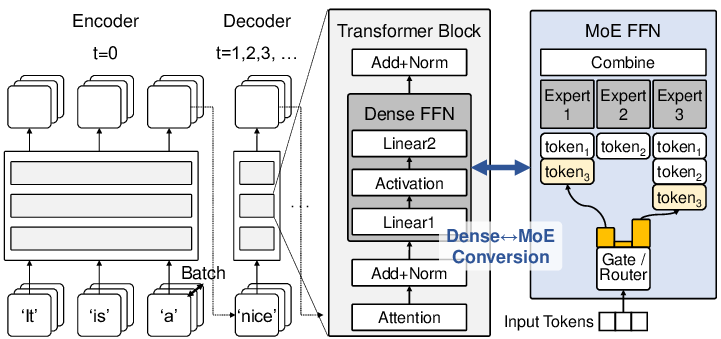
\includegraphics[width=1.0\textwidth]{moe_transformer_block.png}
    \captionof{figure}{So sánh một khối Transformer tiêu chuẩn (trái) và một khối Transformer với lớp MoE (phải). Lớp FFN dày đặc được thay thế bằng một mạng cổng và nhiều chuyên gia FFN thưa thớt.}
    \label{fig:moe_transformer_block}
\end{center}

\subsubsection{Dòng chảy dữ liệu của một token}
Khi một token (được biểu diễn bằng vector $x$) đi vào lớp MoE, quá trình sau sẽ xảy ra:

\paragraph{Bước 1: Định tuyến bởi Mạng cổng (Routing by the Gating Network)}
\begin{itemize}
    \item Token $x$ được đưa vào mạng cổng.
    \item Mạng cổng, thường là một lớp tuyến tính đơn giản, sẽ xuất ra một vector logits có số chiều bằng số chuyên gia ($N$).
    \item Một hàm `softmax` được áp dụng lên vector logits này để tạo ra một phân phối xác suất, $G(x) = (g_1, g_2, \dots, g_N)$, trong đó $g_i$ là "điểm số" hoặc "mức độ tin cậy" mà mạng cổng dành cho chuyên gia thứ $i$.
\end{itemize}

\paragraph{Bước 2: Chọn các Chuyên gia "Top-K"}
\begin{itemize}
    \item Thay vì gửi token đến tất cả các chuyên gia (điều này sẽ làm mất đi tính hiệu quả), hệ thống chỉ chọn ra $k$ chuyên gia có điểm số cao nhất (Top-K routing). Thông thường, $k$ là một số rất nhỏ, ví dụ $k=1$ hoặc $k=2$.
    \item Ví dụ, nếu $k=2$ và chuyên gia thứ 3 và thứ 5 có điểm số cao nhất, thì token này sẽ chỉ được gửi đến hai chuyên gia này. Tất cả các chuyên gia khác sẽ không được kích hoạt cho token này.
\end{itemize}

\paragraph{Bước 3: Xử lý bởi các Chuyên gia}
\begin{itemize}
    \item Token $x$ được đưa qua các mạng FFN của $k$ chuyên gia đã được chọn.
    \item Kết quả đầu ra là $k$ vector: $E_1(x), E_2(x), \dots, E_k(x)$.
\end{itemize}

\paragraph{Bước 4: Tổng hợp có trọng số}
\begin{itemize}
    \item Đầu ra cuối cùng của lớp MoE, $y$, là một tổng có trọng số của đầu ra từ các chuyên gia được chọn. Các trọng số này chính là các điểm số $g_i$ từ mạng cổng đã được chuẩn hóa.
    $$ y = \sum_{i \in \text{TopK}} g_i \cdot E_i(x) $$
\end{itemize}

\subsubsection{Ví dụ: Mixtral 8x7B}
Mô hình Mixtral 8x7B nổi tiếng của Mistral AI là một ví dụ điển hình của MoE.
\begin{itemize}
    \item \textbf{8x7B có nghĩa là gì?} Nó có 8 chuyên gia, mỗi chuyên gia có khoảng 7 tỷ tham số. Tổng số tham số của các lớp MoE là $8 \times 7B = 56B$. Tuy nhiên, đây là số tham số "thưa thớt".
    \item \textbf{Top-2 Routing:} Tại mỗi lớp MoE, mỗi token chỉ được định tuyến đến 2 trong số 8 chuyên gia.
    \item \textbf{Chi phí tính toán:} Do đó, mặc dù tổng số tham số rất lớn, chi phí tính toán để xử lý một token chỉ tương đương với một mô hình dày đặc khoảng $2 \times 7B = 14B$ tham số (cộng với một chi phí nhỏ cho mạng cổng và các lớp khác). Mixtral đạt được chất lượng của một mô hình rất lớn với tốc độ và chi phí của một mô hình nhỏ hơn nhiều.
\end{itemize}
\begin{tcolorbox}[
    title={Các "Chuyên gia" có thực sự chuyên môn hóa không?},
    colback=blue!5!white, colframe=blue!75!black, fonttitle=\bfseries
]
Phép ẩn dụ về "hội đồng chuyên gia" rất hữu ích, nhưng sự chuyên môn hóa của các expert FFN trong thực tế lại trừu tượng hơn nhiều.
\begin{itemize}
    \item \textbf{Không phải là chuyên môn về chủ đề:} Các nghiên cứu đã chỉ ra rằng các expert thường không chuyên môn hóa theo các chủ đề dễ hiểu như "thể thao", "khoa học" hay "lịch sử". Việc định tuyến một token đến expert nào phụ thuộc nhiều vào các đặc trưng trừu tượng của vector biểu diễn của nó.
    \item \textbf{Chuyên môn hóa theo cụm cú pháp/ngữ nghĩa:} Thay vào đó, sự chuyên môn hóa có thể xảy ra ở mức độ thấp hơn. Ví dụ, một số chuyên gia có thể giỏi hơn trong việc xử lý các token là dấu câu, một số khác chuyên về các động từ, một số khác lại tập trung vào các token ở các lớp Transformer cụ thể (ví dụ, các token ở lớp đầu so với lớp cuối).
    \item \textbf{Sự dư thừa có chủ đích:} Có bằng chứng cho thấy các chuyên gia không hoàn toàn độc lập. Thường có sự dư thừa (redundancy) giữa chúng. Điều này có thể là một đặc tính hữu ích, giúp mô hình trở nên mạnh mẽ hơn: nếu một chuyên gia đưa ra kết quả kém, các chuyên gia khác có thể bù đắp.
\end{itemize}
Vì vậy, hãy xem các "chuyên gia" như các \textbf{nhóm tham số (parameter groups)} có thể học được, thay vì các chuyên gia về một lĩnh vực kiến thức cụ thể. Mạng cổng học cách kết hợp các nhóm tham số này một cách tối ưu cho từng token.
\end{tcolorbox}
\subsection{Thách thức trong việc Huấn luyện MoE}
\label{ssec:moe_training_challenges}

Mặc dù rất mạnh mẽ, việc huấn luyện MoE không hề đơn giản và đòi hỏi phải giải quyết một số thách thức đặc thù.

\paragraph{1. Thách thức về sự sụp đổ của việc định tuyến (Routing Collapse)}
Đây là vấn đề lớn nhất của MoE. Nếu không được kiểm soát, mạng cổng sẽ nhanh chóng học được một chiến lược "lười biếng": luôn gửi phần lớn các token đến một hoặc một vài chuyên gia "yêu thích" mà nó cho là tốt nhất.
\begin{itemize}
    \item \textbf{Hậu quả:}
        \begin{enumerate}
            \item \textbf{Lãng phí tham số:} Các chuyên gia khác không nhận được token, do đó không được huấn luyện và trở thành "dead wood". Mô hình MoE khổng lồ sẽ sụp đổ (collapse) thành một mô hình nhỏ hơn nhiều.
            \item \textbf{Mất ổn định huấn luyện:} Gradient sẽ chảy không đều, gây khó khăn cho quá trình tối ưu hóa.
        \end{enumerate}
\end{itemize}

\paragraph{Giải pháp: Hàm Mất mát Cân bằng Tải (Load Balancing Loss)}
Để giải quyết vấn đề này, người ta thêm một \textbf{hàm mất mát phụ trợ (auxiliary loss)} vào hàm mất mát chính của mô hình. Hàm mất mát này được thiết kế để khuyến khích sự phân bổ token đồng đều và thường bao gồm hai thành phần:
\begin{itemize}
    \item \textbf{Một thành phần khuyến khích tầm quan trọng (importance) đồng đều:} Nó phạt nếu tổng các điểm số (logits) mà mạng cổng gán cho mỗi chuyên gia trên toàn bộ một batch là không đồng đều. Điều này đảm bảo mỗi chuyên gia được coi là "quan trọng" như nhau về mặt tổng thể.
    \item \textbf{Một thành phần khuyến khích số lượng token (load) đồng đều:} Nó phạt nếu số lượng token được gửi đến mỗi chuyên gia trong một batch là không đồng đều. Điều này đảm bảo mỗi chuyên gia có "công việc" để làm.
\end{itemize}
Việc cân bằng giữa hàm mất mát chính (ví dụ, cross-entropy) và hàm mất mát phụ trợ này là một trong những khía cạnh nghệ thuật nhất khi huấn luyện các mô hình MoE.

\paragraph{Giải pháp bổ sung: Noisy Top-K Gating}
Một kỹ thuật khác là thêm nhiễu ngẫu nhiên (Gaussian noise) vào logits của mạng cổng trong quá trình huấn luyện.
$$ \text{logits}_{\text{noisy}} = \text{logits}_{\text{original}} + \text{Noise} $$
Nhiễu này buộc mô hình phải "khám phá" (explore) các lựa chọn định tuyến khác nhau thay vì chỉ đi theo con đường quen thuộc, giúp cải thiện sự cân bằng tải một cách tự nhiên.

\paragraph{2. Thách thức về Triển khai và Cơ sở hạ tầng}
\begin{itemize}
    \item \textbf{Bộ nhớ:} Mặc dù chi phí tính toán trên mỗi token thấp, toàn bộ các tham số của tất cả các chuyên gia vẫn phải được tải vào bộ nhớ của GPU, đòi hỏi các hệ thống có bộ nhớ cực lớn.
    \item \textbf{Giao tiếp mạng:} Trong các hệ thống huấn luyện phân tán, các token từ một GPU có thể cần được gửi đến các chuyên gia nằm trên một GPU khác, đòi hỏi băng thông mạng rất cao.
\end{itemize}

\subsection{Tổng kết về MoE}
Mixture-of-Experts là một sự thay đổi mô hình trong cách chúng ta xây dựng các mô hình ngôn ngữ lớn. Nó cho phép chúng ta tách rời \textbf{tổng số tham số} khỏi \textbf{chi phí tính toán trên mỗi token}.

Bằng cách sử dụng các chuyên gia thưa thớt, MoE mở ra một con đường để xây dựng các mô hình có quy mô khổng lồ (hàng nghìn tỷ tham số), có khả năng lưu trữ một lượng kiến thức cực lớn, trong khi vẫn duy trì được tốc độ huấn luyện và suy luận ở mức có thể quản lý được. Đây là một trong những công nghệ nền tảng quan trọng nhất cho thế hệ LLM tiếp theo.

\bigskip
\hrule
\bigskip

\begin{center}
    \textbf{\Large KẾT THÚC CHƯƠNG 4}
\end{center}

\textit{Chương 4 đã là một chuyến đi sâu vào trái tim của NLP hiện đại. Chúng ta đã mổ xẻ kiến trúc Transformer, hiểu được sức mạnh của cơ chế Tự chú ý, và phân loại ba họ mô hình chính -- Encoder-Only, Decoder-Only, và Encoder-Decoder -- đã được sinh ra từ nó. Chúng ta cũng đã khám phá các kỹ thuật tiên tiến cho phép các mô hình này đạt đến quy mô khổng lồ và xử lý ngữ cảnh dài hơn. Về cơ bản, chúng ta đã tìm hiểu cách các "mô hình nền tảng" (foundation models) được xây dựng. Giờ đây, khi đã hiểu rõ cách các mô hình nền tảng khổng lồ này được xây dựng, câu hỏi tiếp theo là: Làm thế nào để chúng ta "thuần hóa" và "chuyên môn hóa" chúng cho các bài toán cụ thể? Chương tiếp theo sẽ tập trung vào các kỹ thuật tinh chỉnh và căn chỉnh, biến những gã khổng lồ đa năng này thành những chuyên gia sắc bén.}